\documentclass{standalone}
\usepackage{tikz}
\usetikzlibrary{patterns, positioning}


\begin{document}
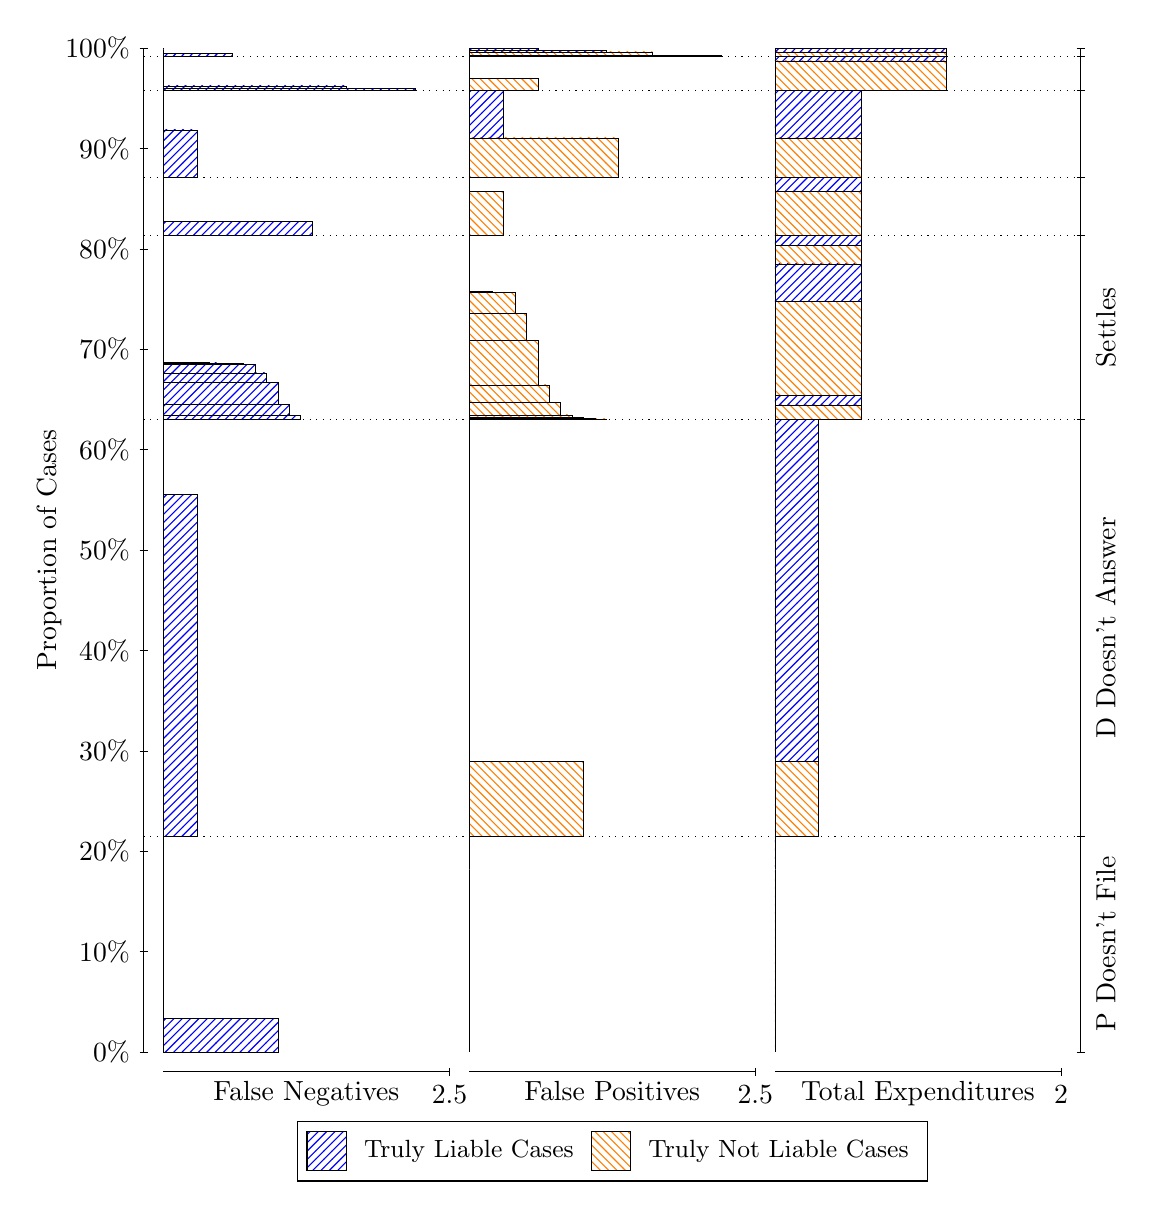
\begin{tikzpicture}
\draw[black, very thin] (1.5,1.75) -- (1.5,14.5);
\node[rotate=90, text=black, anchor=center] at (0.3, 8.125) {Proportion of Cases};
\draw[black, very thin] (1.45,1.75) -- (1.55,1.75);
\node[text=black, anchor=east] at (1.45, 1.75) {0\%};
\draw[black, very thin] (1.45,3.025) -- (1.55,3.025);
\node[text=black, anchor=east] at (1.45, 3.025) {10\%};
\draw[black, very thin] (1.45,4.3) -- (1.55,4.3);
\node[text=black, anchor=east] at (1.45, 4.3) {20\%};
\draw[black, very thin] (1.45,5.575) -- (1.55,5.575);
\node[text=black, anchor=east] at (1.45, 5.575) {30\%};
\draw[black, very thin] (1.45,6.85) -- (1.55,6.85);
\node[text=black, anchor=east] at (1.45, 6.85) {40\%};
\draw[black, very thin] (1.45,8.125) -- (1.55,8.125);
\node[text=black, anchor=east] at (1.45, 8.125) {50\%};
\draw[black, very thin] (1.45,9.4) -- (1.55,9.4);
\node[text=black, anchor=east] at (1.45, 9.4) {60\%};
\draw[black, very thin] (1.45,10.675) -- (1.55,10.675);
\node[text=black, anchor=east] at (1.45, 10.675) {70\%};
\draw[black, very thin] (1.45,11.95) -- (1.55,11.95);
\node[text=black, anchor=east] at (1.45, 11.95) {80\%};
\draw[black, very thin] (1.45,13.225) -- (1.55,13.225);
\node[text=black, anchor=east] at (1.45, 13.225) {90\%};
\draw[black, very thin] (1.45,14.5) -- (1.55,14.5);
\node[text=black, anchor=east] at (1.45, 14.5) {100\%};

\draw[black, very thin] (13.4,1.75) -- (13.4,14.5);
\draw[black, very thin] (13.35,1.75) -- (13.45,1.75);
\node[anchor=west] at (13.35, 1.75) {};
\draw[black, very thin] (13.35,4.4908) -- (13.45,4.4908);
\node[anchor=west] at (13.35, 4.4908) {};
\draw[black, very thin] (13.35,9.7818) -- (13.45,9.7818);
\node[anchor=west] at (13.35, 9.7818) {};
\draw[black, very thin] (13.35,12.123) -- (13.45,12.123);
\node[anchor=west] at (13.35, 12.123) {};
\draw[black, very thin] (13.35,12.855) -- (13.45,12.855);
\node[anchor=west] at (13.35, 12.855) {};
\draw[black, very thin] (13.35,13.962) -- (13.45,13.962);
\node[anchor=west] at (13.35, 13.962) {};
\draw[black, very thin] (13.35,14.394) -- (13.45,14.394);
\node[anchor=west] at (13.35, 14.394) {};
\draw[black, very thin] (13.35,14.5) -- (13.45,14.5);
\node[anchor=west] at (13.35, 14.5) {};

\draw[black, very thin, pattern color=blue, pattern=north east lines] (1.75,1.75) rectangle (3.2033,2.1722);
\draw[black, very thin, pattern color=orange, pattern=north west lines] (1.75,2.1722) rectangle (1.75,4.4908);
\draw[black, very thin, pattern color=blue, pattern=north east lines] (1.75,4.4908) rectangle (2.186,8.8334);
\draw[black, very thin, pattern color=orange, pattern=north west lines] (1.75,8.8334) rectangle (1.75,9.7818);
\draw[black, very thin, pattern color=blue, pattern=north east lines] (1.75,9.7818) rectangle (3.494,9.83);
\draw[black, very thin, pattern color=blue, pattern=north east lines] (1.75,9.83) rectangle (3.3487,9.977);
\draw[black, very thin, pattern color=blue, pattern=north east lines] (1.75,9.977) rectangle (3.2033,10.254);
\draw[black, very thin, pattern color=blue, pattern=north east lines] (1.75,10.254) rectangle (3.058,10.258);
\draw[black, very thin, pattern color=blue, pattern=north east lines] (1.75,10.258) rectangle (3.058,10.373);
\draw[black, very thin, pattern color=blue, pattern=north east lines] (1.75,10.373) rectangle (2.9127,10.484);
\draw[black, very thin, pattern color=blue, pattern=north east lines] (1.75,10.484) rectangle (2.7673,10.492);
\draw[black, very thin, pattern color=blue, pattern=north east lines] (1.75,10.492) rectangle (2.622,10.498);
\draw[black, very thin, pattern color=blue, pattern=north east lines] (1.75,10.498) rectangle (2.4767,10.5);
\draw[black, very thin, pattern color=blue, pattern=north east lines] (1.75,10.5) rectangle (2.3313,10.504);
\draw[black, very thin, pattern color=orange, pattern=north west lines] (1.75,10.504) rectangle (1.75,12.123);
\draw[black, very thin, pattern color=blue, pattern=north east lines] (1.75,12.123) rectangle (3.6393,12.3);
\draw[black, very thin, pattern color=orange, pattern=north west lines] (1.75,12.3) rectangle (1.75,12.855);
\draw[black, very thin, pattern color=blue, pattern=north east lines] (1.75,12.855) rectangle (2.186,13.459);
\draw[black, very thin, pattern color=orange, pattern=north west lines] (1.75,13.459) rectangle (1.75,13.962);
\draw[black, very thin, pattern color=blue, pattern=north east lines] (1.75,13.962) rectangle (4.9473,13.984);
\draw[black, very thin, pattern color=blue, pattern=north east lines] (1.75,13.984) rectangle (4.0753,14.02);
\draw[black, very thin, pattern color=orange, pattern=north west lines] (1.75,14.02) rectangle (1.75,14.394);
\draw[black, very thin, pattern color=blue, pattern=north east lines] (1.75,14.394) rectangle (2.622,14.427);
\draw[black, very thin, pattern color=orange, pattern=north west lines] (1.75,14.427) rectangle (1.75,14.484);
\draw[black, very thin, pattern color=blue, pattern=north east lines] (1.75,14.484) rectangle (1.75,14.5);
\draw[black, very thin, pattern color=orange, pattern=north west lines] (5.6333,1.75) rectangle (5.6333,4.0686);
\draw[black, very thin, pattern color=blue, pattern=north east lines] (5.6333,4.0686) rectangle (5.6333,4.4908);
\draw[black, very thin, pattern color=orange, pattern=north west lines] (5.6333,4.4908) rectangle (7.0867,5.4391);
\draw[black, very thin, pattern color=blue, pattern=north east lines] (5.6333,5.4391) rectangle (5.6333,9.7818);
\draw[black, very thin, pattern color=orange, pattern=north west lines] (5.6333,9.7818) rectangle (7.3773,9.7891);
\draw[black, very thin, pattern color=orange, pattern=north west lines] (5.6333,9.7891) rectangle (7.232,9.7958);
\draw[black, very thin, pattern color=orange, pattern=north west lines] (5.6333,9.7958) rectangle (7.0867,9.8126);
\draw[black, very thin, pattern color=orange, pattern=north west lines] (5.6333,9.8126) rectangle (6.9413,9.8405);
\draw[black, very thin, pattern color=orange, pattern=north west lines] (5.6333,9.8405) rectangle (6.796,10.003);
\draw[black, very thin, pattern color=orange, pattern=north west lines] (5.6333,10.003) rectangle (6.6507,10.221);
\draw[black, very thin, pattern color=orange, pattern=north west lines] (5.6333,10.221) rectangle (6.5053,10.79);
\draw[black, very thin, pattern color=orange, pattern=north west lines] (5.6333,10.79) rectangle (6.36,11.131);
\draw[black, very thin, pattern color=orange, pattern=north west lines] (5.6333,11.131) rectangle (6.2147,11.401);
\draw[black, very thin, pattern color=blue, pattern=north east lines] (5.6333,11.401) rectangle (5.924,11.405);
\draw[black, very thin, pattern color=blue, pattern=north east lines] (5.6333,11.405) rectangle (5.7787,11.407);
\draw[black, very thin, pattern color=blue, pattern=north east lines] (5.6333,11.407) rectangle (5.6333,12.123);
\draw[black, very thin, pattern color=orange, pattern=north west lines] (5.6333,12.123) rectangle (6.0693,12.678);
\draw[black, very thin, pattern color=blue, pattern=north east lines] (5.6333,12.678) rectangle (5.6333,12.855);
\draw[black, very thin, pattern color=orange, pattern=north west lines] (5.6333,12.855) rectangle (7.5227,13.358);
\draw[black, very thin, pattern color=blue, pattern=north east lines] (5.6333,13.358) rectangle (6.0693,13.962);
\draw[black, very thin, pattern color=orange, pattern=north west lines] (5.6333,13.962) rectangle (6.5053,14.118);
\draw[black, very thin, pattern color=orange, pattern=north west lines] (5.6333,14.118) rectangle (5.6333,14.336);
\draw[black, very thin, pattern color=blue, pattern=north east lines] (5.6333,14.336) rectangle (5.6333,14.394);
\draw[black, very thin, pattern color=orange, pattern=north west lines] (5.6333,14.394) rectangle (8.8307,14.402);
\draw[black, very thin, pattern color=orange, pattern=north west lines] (5.6333,14.402) rectangle (7.9587,14.45);
\draw[black, very thin, pattern color=blue, pattern=north east lines] (5.6333,14.45) rectangle (7.3773,14.467);
\draw[black, very thin, pattern color=blue, pattern=north east lines] (5.6333,14.467) rectangle (6.5053,14.5);
\draw[black, very thin, pattern color=orange, pattern=north west lines] (9.5167,1.75) rectangle (9.5167,4.0686);
\draw[black, very thin, pattern color=blue, pattern=north east lines] (9.5167,4.0686) rectangle (9.5167,4.4908);
\draw[black, very thin, pattern color=orange, pattern=north west lines] (9.5167,4.4908) rectangle (10.062,5.4391);
\draw[black, very thin, pattern color=blue, pattern=north east lines] (9.5167,5.4391) rectangle (10.062,9.7818);
\draw[black, very thin, pattern color=orange, pattern=north west lines] (9.5167,9.7818) rectangle (10.607,9.9683);
\draw[black, very thin, pattern color=blue, pattern=north east lines] (9.5167,9.9683) rectangle (10.607,10.087);
\draw[black, very thin, pattern color=orange, pattern=north west lines] (9.5167,10.087) rectangle (10.607,11.282);
\draw[black, very thin, pattern color=blue, pattern=north east lines] (9.5167,11.282) rectangle (10.607,11.759);
\draw[black, very thin, pattern color=orange, pattern=north west lines] (9.5167,11.759) rectangle (10.607,11.996);
\draw[black, very thin, pattern color=blue, pattern=north east lines] (9.5167,11.996) rectangle (10.607,12.123);
\draw[black, very thin, pattern color=orange, pattern=north west lines] (9.5167,12.123) rectangle (10.607,12.678);
\draw[black, very thin, pattern color=blue, pattern=north east lines] (9.5167,12.678) rectangle (10.607,12.855);
\draw[black, very thin, pattern color=orange, pattern=north west lines] (9.5167,12.855) rectangle (10.607,13.358);
\draw[black, very thin, pattern color=blue, pattern=north east lines] (9.5167,13.358) rectangle (10.607,13.962);
\draw[black, very thin, pattern color=orange, pattern=north west lines] (9.5167,13.962) rectangle (11.697,14.336);
\draw[black, very thin, pattern color=blue, pattern=north east lines] (9.5167,14.336) rectangle (11.697,14.394);
\draw[black, very thin, pattern color=orange, pattern=north west lines] (9.5167,14.394) rectangle (11.697,14.45);
\draw[black, very thin, pattern color=blue, pattern=north east lines] (9.5167,14.45) rectangle (11.697,14.5);
\draw[black, dotted] (1.5,4.4908) -- (13.4,4.4908);
\draw[black, dotted] (1.5,9.7818) -- (13.4,9.7818);
\draw[black, dotted] (1.5,12.123) -- (13.4,12.123);
\draw[black, dotted] (1.5,12.855) -- (13.4,12.855);
\draw[black, dotted] (1.5,13.962) -- (13.4,13.962);
\draw[black, dotted] (1.5,14.394) -- (13.4,14.394);
\draw[black, very thin] (1.75,1.5) -- (5.3833,1.5);
\node[text=black, anchor=north] at (3.5667, 1.5) {False Negatives};
\draw[black, very thin] (5.3833,1.45) -- (5.3833,1.55);
\node[text=black, anchor=north] at (5.3833, 1.45) {2.5};

\draw[black, very thin] (5.6333,1.5) -- (9.2667,1.5);
\node[text=black, anchor=north] at (7.45, 1.5) {False Positives};
\draw[black, very thin] (9.2667,1.45) -- (9.2667,1.55);
\node[text=black, anchor=north] at (9.2667, 1.45) {2.5};

\draw[black, very thin] (9.5167,1.5) -- (13.15,1.5);
\node[text=black, anchor=north] at (11.333, 1.5) {Total Expenditures};
\draw[black, very thin] (13.15,1.45) -- (13.15,1.55);
\node[text=black, anchor=north] at (13.15, 1.45) {2};

\node[text=black, centered, rotate=90] at (13.72, 3.1204) {P Doesn't File};
\node[text=black, centered, rotate=90] at (13.72, 7.1363) {D Doesn't Answer};
\node[text=black, centered, rotate=90] at (13.72, 10.952) {Settles};





\draw (7.449999999999999,1.5) node[draw=none] (baseCoordinate) {};
\begin{scope}[align=center]
        \matrix[scale=0.5, draw=black, below=0.5cm of baseCoordinate, nodes={draw}, column sep=0.1cm]{
            \node[rectangle, draw, minimum width=0.5cm, minimum height=0.5cm, pattern color=blue, pattern=north east lines] {}; &
            \node[draw=none, font=\small, text=black] (B) {Truly Liable Cases}; &
            \node[rectangle, draw, minimum width=0.5cm, minimum height=0.5cm, pattern color=orange, pattern=north west lines] {}; &
            \node[draw=none, font=\small, text=black] (B) {Truly Not Liable Cases}; \\
            };
\end{scope}

\end{tikzpicture}
\end{document}